\documentclass{sig-alternate}

\usepackage{amsmath,mathtools,nccmath}
\usepackage{paralist}
\usepackage{tikz}
\usetikzlibrary{matrix,arrows,shapes,calc}

\newtheorem{example}{Example}
\newtheorem{definition}{Definition}
\newtheorem{theorem}{Theorem}

\newcommand{\ifthenelse}[3]{\mathbf{if}\ #1\ \mathbf{then}\ #2\ \mathbf{else}\ #3}
\newcommand{\pvec}[1]{\vec{#1}\mkern2mu\vphantom{#1}} %for primed vector (by egreg)
\newcommand{\abs}{\ensuremath{\mathrm{abs}}}
\newcommand{\sign}{\ensuremath{\mathrm{sign}}}


\begin{document}

\title{Evaluating PALS with SMT on a Distributed Nonlinear Airplane Turning Controller
%\titlenote{For use with ACM\_PROC\_ARTICLE-SP.CLS. Supported by ACM.}
}

\numberofauthors{3}
\author{
Kyungmin Bae, Sicun Gao, Edmund M. Clarke\\
\affaddr{Department of Computer Science}\\
\affaddr{Carnegie Mellon University}
}

\maketitle
\begin{abstract}
We evaluate the performance of SMT-based analysis on a distributed
nonlinear aircraft controller. Such a model has been studied using
techniques from ..., but there are limitations such as... We show how
to generate SMT formulas to solve problems in the PALS framework and
evaluate the scalability of state-of-the-art SMT solving techniques on
these problems. We also give directions for improvement on SMT for
handling more general properties like ....
\textbf{TO BE WRITTEN}
\end{abstract}

%%%%
%%%%
\section{Introduction}

\textbf{TO BE WRITTEN}

\newpage
..

\newpage

%%%
\subsection{Related Work}

\newpage



%%%%
%%%%
\section{Preliminaries}

%%%
\subsection{Multirate PALS} 

The Multirate PALS (``physically asynchronous,  logically synchronous'') 
methodology \cite{pals-rtss09,mr-pals-journal,pals-tcs}
aims at reducing the system complexity 
of \emph{virtually synchronous}  cyber physical systems (CPS),
such as airplanes and cars,
implemented as a network of multirate distributed components but essentially designed in a synchronous way.
%
The design and verification of a virtually synchronous CPS
is challenging  due to
clock skews,
execution times, 
network delays, and asynchronous communication,
plus the state space explosion caused by the system's concurrency. 
%
Multirate PALS can reduce
the design and verification of a virtually synchronous CPS to
that of its much simpler synchronous counterpart,
provided that the underlying infrastructure provides bounds $\Gamma$
on the skews of the local clocks, 
execution times,  and network delays. 
%
Given a synchronous design $\mathcal{E}$ and a global period $T$,
Multirate PALS generates
the corresponding distributed asynchronous 
design $\mathcal{A}(\mathcal{E}, T, \Gamma)$
in which both $\mathcal{E}$ and $\mathcal{A}(\mathcal{E}, T, \Gamma)$
satisfy the same temporal logic properties \cite{mr-pals-journal,pals-tcs}.
%
%By simply designing and verifying a synchronous model $\mathcal{E}$,
%Multirate PALS %can automatically 
%gives the \emph{correct-by-construction}  
%implementation  $\mathcal{A}(\mathcal{E}, T, \Gamma)$.



The multirate synchronous model $\mathcal{E}$ 
is formally specified as
a synchronous composition of a set of  nondeterministic state machines \cite{pals-tcs}.
%
A \emph{typed machine} with $n$ input ports and $m$ output ports
is a tuple $M = (D_i,S,D_o,\delta_M)$,
where
$D_i = D_{i_1} \times \cdots \times D_{i_n}$ is an input set 
(a value to the $k$-th \emph{input port}  is an element of $D_{i_k}$ for $1 \leq k \leq n$), %
$S$ is a finite set of states,
$D_o =D_{o_1} \times \cdots \times D_{o_m}$ is an output set
(a value from the $j$-th \emph{output port} is an element of $D_{o_j}$ for $1 \leq j \leq m$), %
and
$\delta_M \subseteq (D_i \times S) \times (S \times D_o)$ is a %total 
transition relation of $M$.
A collection of typed machines \emph{with different rates}
can be composed into a \emph{multirate machine ensemble} $\mathcal{E}$,
using  a \emph{wiring diagram} that connects  the input and output ports of the machines,
as illustrated in Figure~\ref{fig:ensemble}.
The period of a slow machine is a multiple of the period of a connected fast machine,
and the physical environments are 
assumed to be already integrated with their controllers (see below).


\begin{figure}
\centering
\includegraphics[clip=true,trim=0.3cm 0.4cm 0.3cm 0.4cm,width=1.0\columnwidth]{ensemble.pdf}    
\caption{A multirate machine ensemble $\mathcal{E}$.
%$M_1$ and $M_2$ are slow machines, and 
%%%$M_3$, $M_4$, and $M_5$ are fast machines.
%$\mathit{env}_4$ and $\mathit{env}_5$ are local physical environments 
%of $M_4$ and $M_5$, respectively.
}  \label{fig:ensemble}
\end{figure}



The transitions of all components in an ensemble $\mathcal{E}$
are performed at the same time in lockstep for each iteration.
Each fast machine $M_f$ in $\mathcal{E}$ is \emph{slowed down} 
by performing $k = \mathit{rate}(f)$ internal transitions  in one synchronous step.
A $k$-tuple of outputs from $M_f$  is transformed to 
a single value (e.g., the last value) %or the average of the $k$ values
for a slow machine,
and a single input  from a slow machine
is transformed to a $k$-tuple of inputs for $M_f$
(e.g., a $k$-tuple $(d, d, d, d)$ from a value $d$).
%(e.g., a $k$-tuple $(d, \bot, \ldots, \bot)$ for some ``don't care'' value $\bot$).
%
When a machine has a ``feedback'' wire connected to itself or to another component,
the output becomes an input of the destination component in the \emph{next} iteration.
That is,
the \emph{synchronous composition}  of an ensemble $\mathcal{E}$
is equivalent to a single machine $M_\mathcal{E}$
whose state consists of the states of its subcomponents
and the feedback outputs \cite{mr-pals-journal,pals-tcs}.
For example, 
the synchronous composition $M_\mathcal{E}$ 
of the ensemble $\mathcal{E}$ in Figure~\ref{fig:ensemble} 
is the machine given by the outer box. 
%Notice that $M_\mathcal{E}$ can appear as a component 
%in another multirate ensemble, resulting in hierarchical multirate systems.

%Since a fast machine performs $k$ internal transitions 
%one synchronous step,
%a $k$-tuple of outputs from the fast machine
%must be transformed to a single input (e.g., the last value, or the average of the $k$ values)
%to be read by a slow component.
%Similarly,
%a single output from a slow component must be transformed 
%to a $k$-tuple of inputs for a fast component
%(e.g., 
%a $k$-tuple $(d, \bot, \ldots, \bot)$ for some ``don't care'' value $\bot$).
%An \emph{input adaptor} 
%$\alpha=\{\alpha_j: D'_j \rightarrow D_{i_j}\}_{j\in\{1,\ldots, n\}}$
%for a typed machine $M = (D_i, S, D_o, \delta_M)$
%is a family of functions which determine a desired  value 
%$\alpha_j(d_j) \in D_{i_j}$ for each input 
%port $j$  from an output $d_j \in D_{j}'$
%of another typed machine.


The physical environments of controllers
are specified as periodic dynamic systems \cite{ftscs-journal}.
%
A controller $M$ is a ``periodic'' component 
that collects the state of  its physical environment  $E_M$ using its sensors,
 and has an effect on $E_M$ through its  actuators.
A state of the physical environment $E_M$ 
is given by a tuple $\vec{v} = (v_1,\ldots,v_l) \in \mathbb{R}^l$ 
of its physical parameters $\vec{x} = (x_1, \ldots,x_l)$.
The behavior of $E_M$
is modeled using differential equations that specify \emph{trajectories} 
$\tau_1, \ldots, \tau_l$ of the parameters $\vec{x}$.
A \emph{trajectory} \cite{lynch2003hybrid} of duration $T \in \mathbb{R}_{\geq 0}$ is a function $\tau : [0,T] \rightarrow \mathbb{R}$
that defines the 
continuous behavior of a physical parameter.
%
Let  $\mathcal{T}_T$ denote
the set of all trajectories of 
duration $T$,
and $\vec{\tau}(t) = (\tau_1(t),\ldots,\tau_l(t))$ for a tuple %of trajectories 
$\vec{\tau} = (\tau_1,\ldots,\tau_l) \in \mathcal{T}_T^l$.

A \emph{periodic dynamic system} $E_M = (C, P, T, \Lambda)$ 
specifies all possible trajectories of its parameters $\vec{x}$
during period $T$, % \in \mathbb{R}_{>0}
where:
 \begin{inparaenum}[(i)]
	\item $C$ is a set of \emph{control commands}, representing
          ``actuator outputs'' from %the controller 
          $M$;
	\item $P \subseteq \mathbb{R}^l$ is a set of all possible values 
          of the ``physical 
          parameters'' $\vec{x} = (x_1, \ldots, x_l)$ 
          of  $E_M$; and
	\item $\Lambda \subseteq (C \times P) \times \mathcal{T}_{T}^l$
	is a \emph{physical transition relation} in which
	%that defines possible trajectories of the parameters $\vec{x}$.
	%By definition, 
	$((a, \vec{v}),  \vec{\tau}) \in \Lambda$
	 iff for a control command $a \in C$, % of the controller $M$,
	$E_M$'s physical state gives the trajectory 
	$\vec{\tau} \in \mathcal{T}_{T}^l$ during period $T$
	from a physical state $\vec{v} \in P$
	with $\vec{\tau}(0) = \vec{v}$ at the beginning of a period.
\end{inparaenum}
%
For example,
a physical transition in Figure~\ref{fig:physical-transition} 
defines a trajectory $\tau_i$
from the value $v_i$ to $v_{i+1}$
 according to the control command $a_i$ 
from $M$ during each period.






\begin{figure}
\centering
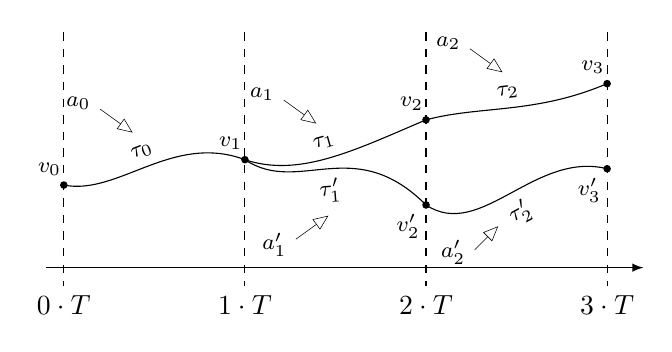
\begin{tikzpicture}[scale=2.3]
%baseline
\draw[-latex,thin] (-0.1,0) -- (3.2,0);
\foreach \x in {0,1,2,3}
\draw[shift={(\x,0)},thin,dashed] (0,1.3) -- (0,-0.1) node[below] { $\x\cdot T$};
%curves
\begin{scope}[yshift=7pt,font=\footnotesize]
\filldraw (0,0.21) circle (0.5pt) node[above,xshift=-1.2ex] {$v_0$};
\draw (0,0.21) .. controls (0.3,0.15) and (0.6,0.5) .. node[above,sloped] (t0) {$\tau_0$} (1,0.35);
\draw[-open triangle 45,very thin] ($(t0.north) + (-0.2,0.15)$) node[left,yshift=2pt] {$a_0$} -- ($(t0.north) + (-0.02,0.02)$);
	\filldraw (1,0.35) circle (0.5pt) node[above,xshift=-1.2ex] {$v_1$};
	\draw (1,0.35) .. controls (1.3,0.25) and (1.6,0.4) .. node[above,sloped] (t1) {$\tau_1$} (2,0.57);
	\draw[-open triangle 45,very thin] ($(t1.north) + (-0.2,0.15)$) node[left,yshift=2pt] {$a_1$} -- ($(t1.north) + (-0.02,0.02)$);
		\filldraw (2,0.57) circle (0.5pt) node[above,xshift=-1.2ex] {$v_2$};
		\draw (2,0.57) .. controls (2.3,0.65) and (2.6,0.6) .. node[above,sloped] (t2) {$\tau_2$} (3,0.77);
		\draw[-open triangle 45,very thin] ($(t2.north) + (-0.2,0.15)$) node[left,yshift=2pt] {$a_2$} -- ($(t2.north) + (-0.02,0.02)$);
			\filldraw (3,0.77) circle (0.5pt) node[above,xshift=-1.2ex] {$v_3$};
	\draw (1,0.35) .. controls (1.3,0.15) and (1.6,0.5) .. node[below,sloped] (t1') {$\tau_1'$} (2,0.1);
	\draw[-open triangle 45,very thin] ($(t1'.south) + (-0.2,-0.15)$) node[left,yshift=-2pt] {$a_1'$} -- ($(t1'.south) + (-0.02,-0.02)$);
		\filldraw (2,0.1) circle (0.5pt) node[below,xshift=-1.5ex] {$v_2'$};
		\draw (2,0.1) .. controls (2.3,-0.1) and (2.6,0.4) .. node[below,sloped] (t2'){$\tau_2'$} (3,0.3);
		\draw[-open triangle 45,very thin] ($(t2'.west) + (-0.15,-0.15)$) node[left,yshift=-1pt] {$a_2'$} -- ($(t2'.west) + (-0.02,-0.02)$);
			\filldraw (3,0.3) circle (0.5pt) node[below,xshift=-1.5ex] {$v_3'$};;;
\end{scope}
\end{tikzpicture}
\caption{A periodic dynamic system $E_M$,
where
$((a_0,v_0), \tau_0) \in \Lambda$, 
$((a_1,v_1), \tau_1) \in \Lambda$, 
$((a_1',v_1), \tau_1') \in \Lambda$, 
%$((a_2,v_2), \tau_2) \in \Lambda$, 
%$((a_2',v_2), \tau_2') \in \Lambda$, 
etc.
}
\label{fig:physical-transition}
\end{figure}





A controller machine $M = (D_i, S, D_o,\delta_{M})$ is considered as 
a \emph{nondeterministic} typed
machine that is
parameterized  by any possible \emph{observable}
behavior of %its physical environment 
$E_M  = (C, P, U, \Lambda)$.
Each state $s \in S$ of $M$ provides
the current control command %of $M$ 
to $E_M$,
denoted by $\pi_C(s) \in C$, and
the ``observed'' physical state by $M$
from a physical state  $\vec{v} \in P$ of $E_M$,
denoted by $\pi_P(s) = \pi_S(\vec{v})$.
%
That is,
the control command $\pi_C(s)$ to $E_M$ is given based on the current state $s$ of $M$,
and
the ``observable'' physical parameters $\pi_S(\vec{v})$ of $E_M$ 
are observed as $\pi_P(s)$ by $M$.
%\footnote{A controller $M$
%is assumed to be tightly integrated with its physical environment $E_M$,
%and thus $M$ can observe or affect $E_M$  immediately;
%for ``remote'' sensors and actuators, % not tightly integrated,
%they  can be considered as parts of another
%controller that communicates with $M$ via a network \cite{ftscs-journal}.}
%
The \emph{environment restriction} %of $M$ by $E_M$ 
is then defined as the machine
$M \restriction E_M = (D_i, S \times P, D_o, \delta_{M \restriction E_M})$,
where 
its transition relation 
$\delta_{M \restriction E_M}$ is constrained by the behavior of $E_M$: i.e.,
%
%a transition 
$((\vec{i}, (s,\vec{v})), ((s',\pvec{v}'), \vec{o}) ) \in \delta_{M \restriction E_M}$ holds
iff:

\begin{itemize}
	\item the $M$'s transition $( (\vec{i}, s), (s', \vec{o}) ) \in \delta_{M}$ holds;
	\item $\pi_P(s) = \pi_S(\vec{v})$ and $\pi_P(s') = \pi_S(\pvec{v}')$ hold; and
	\item the $E_M$'s physical transition 
	$((\pi_C(s), \vec{v}),  \vec{\tau} ) \in \Lambda$
	holds 
	from the current physical state $\vec{v} = \vec{\tau}(0)$ 
	to the next physical state $\pvec{v}' = \vec{\tau}(T)$ during period $T$
	(in other words, the next physical state $\pvec{v}'$ of $E_M$ is 
	reachable from $\vec{v}$  through some trajectory $\vec{\tau}$
	of  $E_M$ based on the current control command $\pi_C(s)$).
\end{itemize}










%%%
\subsection{Delta-Complete SMT}

\textbf{To be written by Sean}
\newpage


%%%%
%%%%
\section{CPS for Turning an Airplane}

This section illustrates a distributed hybrid system
for turning an airplane to an angle specified by a pilot,
through a distributed control system to move the ailerons and the rudder 
of the airplane
in a synchronous way.
An aileron is a movable surface attached to  each wing, and a rudder is a movable surface attached to the vertical tail.
%
The controllers 
for the ailerons and the rudder operate at different rates,
and the main controller orchestrates the sub-controllers 
to achieve a smooth turn
according to a specified goal angle.
%
The continuous dynamics of the turning control system
is governed by \emph{nonlinear} differential equations
that involve the angles of the ailerons and the rudder.




An airplane typically makes a turn by operating its two ailerons in opposite directions.
The difference between the lift forces in the left and the right wings
then makes the airplane roll toward a desired direction, 
so that the airplane moves in a circular motion 
because of  the centripetal lift force 
generated by the two wings.
However, the rolling of the airplane also causes
\emph{adverse yaw}, making the airplane sideslip in the opposite direction of a roll.
This undesirable side effect can be countered by 
generating the opposing side lift force on the vertical tail
by moving the rudder of the airplane.
To make a \emph{coordinated turn} effectively, the yaw angle $\beta$ should
always stay at $0^\circ$
during a turn.




Under some simplifying assumptions,%
\footnote{E.g., the wings of the airplane have no dihedral angle, 
the speed $v$ of the airplane is constant, 
the altitude does not change, there is no turbulence, etc.}
the direction angle $\psi$, the roll angle $\phi$, and the yaw angle $\beta$
can be modeled by the following nonlinear differential equations 
including 
the angle $x_L$ of the left aileron,
the angle $x_R$ of the right aileron, and 
the angle $x_V$ of the rudder
\cite{ftscs-journal}:
%
\begin{align}
\frac{\mathrm{d}\psi}{\mathrm{d}t} &= (g / v) * \tan \phi
\label{eq:dir}
\\
(\frac{\mathrm{d}\phi}{\mathrm{d}t})^2 &=
(C_{l,w} \cdot x_R - C_{l,w} \cdot x_L) / (W * L_{\mathit{Wing}})
\label{eq:roll}
\\
(\frac{\mathrm{d}\beta}{\mathrm{d}t})^2 &=
\begin{multlined}[t]
C_d \cdot (C_{l,w} \cdot x_R - C_{l,w} \cdot x_L) / (W * L_{\mathit{Wing}})
\\
 \;+\; C_{l,v} \cdot x_V / (W \cdot L_{\mathit{Aircraft}})
\end{multlined}
 \label{eq:yaw}
\end{align}
%
where $(\frac{\mathrm{d}\phi}{\mathrm{d}t})^2 = f(t)$
means that 
$\frac{\mathrm{d}\phi}{\mathrm{d}t} = \sqrt{f(t)}$ if $f(t) \geq 0$,
and
$\frac{\mathrm{d}\phi}{\mathrm{d}t} = - \sqrt{- f(t)}$ if $f(t) < 0$.
In the equation, $g$ is the gravity constant, $v$ is the speed of the airplane,
$W$ is the mass of the airplane, 
 $L_{\mathit{Wing}}$ is the length of the left or the right wing,
 $L_{\mathit{Aircraft}}$ is the length of the airplane,
 $C_{l,w}$ is the lift constant for the horizontal wings,
 $C_{l,v}$ is the lift constant for the vertical tail wing,
 and  $C_d$ is the drag ratio.%
 \footnote{The values of the constants  $C_{l,w}$,  $C_{l,v}$, and $C_d$
 depend on the shape of the wing or the aircraft.}

 




Using the Multirate PALS methodology,
we only specify  a synchronous model,
namely,  a multirate ensemble $\mathcal{E}$ that consists of 
the main controller and the three sub-controllers.
These controllers in $\mathcal{E}$ defines 
the system's \emph{discrete} behavior,
while their local physical environments
%given by periodic dynamic systems,
defines the system's continuous behavior.
%
Multirate PALS then generates
the \emph{correct-by-construction}   
implementation  
$\mathcal{A}(\mathcal{E}, T, \Gamma)$,
given a global period $T$ and performance bounds 
$\Gamma$ on the network infrastructure.
%
The synchronous model $\mathcal{E}$ %in this section
is adapted from \cite{ftscs-journal} 
for precisely specifying \emph{immediate correlation}
between the physical environments of the controllers.
%
The architecture of the system is illustrated in Figure~\ref{fig:airplane-ctrl}.

\begin{figure}
\centering
\tikzstyle{comp}=[draw,thick,rounded corners=4pt,text centered,execute at begin node=\small]
\tikzstyle{env}=[draw,dashed,rounded corners=4pt,text centered,execute at begin node=\small]
\tikzstyle{conn}=[thick,-latex,font=\scriptsize]
\tikzstyle{envconn}=[very thin,-open triangle 45,font=\scriptsize]
\begin{tikzpicture}[scale=0.9,every node/.style={transform shape}] 
%components
\node (main) [comp,text width=10ex,minimum height=36ex] 
	{{Main\\ controller} ($60\, \mathrm{ms}$, $\mathit{rate}$ = $1$)}; 
\path (main.east |- main.north) + (17ex,-5.5ex) node (left) [comp,text width=12.5ex,minimum height=11ex] 
	{{Left wing\\ subcontroller}\\ ($15\, \mathrm{ms}$, $\mathit{rate}$ = $4$)}; 
\path (main.east) + (17ex,0) node (vert) [comp,text width=12.5ex,minimum height=11ex] 
	{{Rudder\\ subcontroller}\\ ($20\, \mathrm{ms}$, $\mathit{rate}$ = $3$)}; 
\path (main.east |- main.south) + (17ex,5.5ex) node (right) [comp,text width=12.5ex,minimum height=11ex] 
	{{Right wing\\ subcontroller}\\ ($15\, \mathrm{ms}$, $\mathit{rate}$ = $4$)}; 
%comp connections
\draw [conn,latex-] (main.west |- main.north) + (3ex,0)-- node{ }+(3ex,3ex) node[above] {$\mathit{goal}_\psi$};
\draw [conn] (main.east |- main.north) + (-3ex,0)-- node{ }+(-3ex,3ex) node[above] {$\psi$};
\draw[conn] ($(main.east |- left)+(0,1ex)$) -- node[above] {$\mathit{goal}_L$} ($(left.west |- left)+(0,1ex)$);
\draw[conn] ($(left.west |- left)+(0,-1ex)$) -- node[below] {$a_L$} ($(main.east |- left)+(0,-1ex)$);
\draw[conn] ($(main.east |- vert)+(0,1ex)$) -- node[above] {$\mathit{goal}_V$} ($(left.west |- vert)+(0,1ex)$);
\draw[conn] ($(left.west |- vert)+(0,-1ex)$) -- node[below] {$a_V$} ($(main.east |- vert)+(0,-1ex)$);
\draw[conn] ($(main.east |- right)+(0,1ex)$) -- node[above] {$\mathit{goal}_R$} ($(left.west |- right)+(0,1ex)$);
\draw[conn] ($(left.west |- right)+(0,-1ex)$) -- node[below] {$a_R$} ($(main.east |- right)+(0,-1ex)$);
%physical envs
\path (main.west) + (-9.5ex,0ex) node (main-env) [env,text width=6ex,minimum height=36ex] 
	{$E_\mathit{Main}$}; 
\path (left.east) + (14ex,0ex) node (left-env) [env,text width=8ex,minimum height=11ex] 
	{$E_\mathit{Left}$}; 
\path (vert.east) + (14ex,0ex) node (vert-env) [env,text width=8ex,minimum height=11ex] 
	{$E_\mathit{Rudder}$}; 
\path (right.east) + (14ex,0ex) node (right-env) [env,text width=8ex,minimum height=11ex] 
	{$E_\mathit{Right}$}; 
%physical env conns
\draw[envconn] ($(main-env.east |- main-env.north)+(0,-8ex)$)
	-- node[above] {$\psi$} ($(main.west |- main-env.north)+(0,-8ex)$);
\draw[envconn] (main-env.east)
	-- node[above] {$\phi$} (main.west);
\draw[envconn] ($(main-env.east |- main-env.south)+(0,8ex)$)
	-- node[above] {$\beta$} ($(main.west |- main-env.south)+(0,8ex)$);
\draw[envconn] ($(left.east |- left-env)+(0,1ex)$) 
	-- node[above] {$\mathit{rate}_L$} ($(left-env.west |- left-env)+(0,1ex)$);
\draw[envconn] ($(left-env.west |- left-env)+(0,-1ex)$) 
	-- node[below] {$x_L$} ($(left.east |- left-env)+(0,-1ex)$);
\draw[envconn] ($(vert.east |- vert-env)+(0,1ex)$) 
	-- node[above] {$\mathit{rate}_\mathit{V}$} ($(vert-env.west |- vert-env)+(0,1ex)$);
\draw[envconn] ($(vert-env.west |- vert-env)+(0,-1ex)$) 
	-- node[below] {$x_V$} ($(vert.east |- vert-env)+(0,-1ex)$);
\draw[envconn] ($(right.east |- right-env)+(0,1ex)$) 
	-- node[above] {$\mathit{rate}_\mathit{R}$} ($(right-env.west |- right-env)+(0,1ex)$);
\draw[envconn] ($(right-env.west |- right-env)+(0,-1ex)$) 
	-- node[below] {$x_R$} ($(right.east |- right-env)+(0,-1ex)$);
\end{tikzpicture}
\caption{The airplane turning control system.} \label{fig:airplane-ctrl}
\end{figure}

\subsection{The Aileron and Rudder Controllers}

A sub-controller receives a desired angle of the wing
from the main controller,
and gradually moves the surface of the wing toward the goal angle.
The continuous change of the angle is modeled by its physical environment.
For example, 
the left wing sub-controller receives $\mathit{goal}_L$ from the main controller, 
and sets the moving rate $\mathit{rate}_L$
  for the physical environment $E_\mathit{Left}$
(that is less than or equal to the maximal rate $\max_L$).
%
Meanwhile, the wing angle $x_L$ in $E_\mathit{Left}$  changes according to the differential equation
$\frac{\mathrm{d} x_L}{\mathrm{d}t} = \mathit{rate}_L$ during its $15\,\mathrm{ms}$ period.
%
The right wing and the rudder sub-controllers are similar,
except their periods and the maximal rates.

The left wing sub-controller  can be specified 
as the typed machine 
$M_\mathit{Left} = (\mathbb{R}, \mathbb{R}^2, \mathbb{R}, \delta_{\mathit{Left}})$.
The machine $M_\mathit{Left}$ has one input port to receive $\mathit{goal}_L \in \mathbb{R}$,
and one output port to report the observed angle. % of the wing.
A state $(\mathit{rate}_L, a_L) \in \mathbb{R}^2$ is a pair of the current rate $\mathit{rate}_L$ and the observed angle $a_L$.
A transition $((\mathit{goal}_L, (r, a)), ((r', a'),a)) \in  \delta_{\mathit{Left}}$
holds iff 
\[
r' = 
\begin{cases}
\min((\mathit{goal}_L - a) / 15, \max_L)  & \mbox{if } \mathit{goal}_L \geq a
\\
- \min((a - \mathit{goal}_L) / 15, \max_L) & \mbox{if } \mathit{goal}_L < a,
\end{cases}
\]
and $a' \in \mathbb{R}$ is the \emph{next}  observed angle after $15\,\mathrm{ms}$ elapsed,
determined by the physical environment $E_\mathit{Left}$.

The periodic dynamic system 
$E_\mathit{Left} = (\mathbb{R}, \mathbb{R}, 15\,\mathrm{ms}, \Lambda_\mathit{Left})$
has the control command set $\mathbb{R}$ for the moving rate $\mathit{rate}_L$,
and the state set $\mathbb{R}$ for the angle of the left wing.
The physical transition 
$( (\mathit{rate}_L, a_L), x_L ) \in \Lambda_{E_\mathit{Left}}$ holds
iff there exists a trajectory $x_L \in \mathcal{T}_{15}$ such that
$\frac{\mathrm{d} x_L}{\mathrm{d}t} = \mathit{rate}_L$ and $x_L(0) = a_L$
(i.e., the wing angle  $x_L$ changes from the current angle $x_L(0) = a_L$
during a $15\,\mathrm{ms}$ period according to the differential 
equation $\frac{\mathrm{d} x_L}{\mathrm{d}t} = \mathit{rate}_L$).

The combined behavior is then given by the environment restriction 
$M_\mathit{Left} \restriction E_\mathit{Left} = (\mathbb{R}, \mathbb{R}^2 \times \mathbb{R}, \mathbb{R}, \delta_{M_\mathit{Left} \restriction E_\mathit{Left}})$.
A transition 
$((\mathit{goal}_L, (r, a, a))), ((r',a', a'), a) ) 
\in \delta_{M_\mathit{Left} \restriction E_\mathit{Left}}$ 
is defined iff
the transition $( (\mathit{goal}_L, (r,a)), ((r',a'),a) ) \in \delta_{\mathit{Left}}$
of $M_\mathit{Left}$
and the physical transition 
$((r, a), x_L) \in \Lambda_{\mathit{Left}}$ of $E_\mathit{Left}$ hold
with the current angle $x_L(0) = a$ and the next angle $x_L(15) = a'$,
where the control commands to $E_\mathit{Left}$ are defined by the projection function $\pi_C(r,a) = r$,
and the observed parameters of $E_\mathit{Left}$ by $M_\mathit{Left}$
are given by the projection functions $\pi_P(r,a) = a$ and $\pi_S(a) = a$.
Notice that $M_\mathit{Left}$ is nondeterministic
since the next observed angle $a'$ is not specified,
whereas
$M_\mathit{Left} \restriction E_\mathit{Left}$ is deterministic.




\subsection{The Main Controller}

The main controller $M_\mathit{Main}$ receives 
a desired direction of the airplane (specified by the pilot),
and determines the new surface angles of the sub-controllers
for a coordinated turn. 
%
The direction angle $\psi$, the roll angle $\phi$, and the yaw angle $\beta$,
governed by the nonlinear differential equations (\ref{eq:dir}--\ref{eq:yaw}),
consist in the physical environment $E_\mathit{Main}$.
For each step, the main controller receives the goal direction
$\mathit{goal}_\psi$ from the pilot 
and the observed surface angles $(a_L, a_V, a_R)$
from the aileron and the rudder sub-controllers,
and then sends the new goal angles 
$(\mathit{goal}_L, \mathit{goal}_V, \mathit{goal}_R)$ to the sub-controllers,
based on the current observed position angles $(\psi, \phi, \beta)$.


The position angles $\psi$, $\phi$, and $\beta$ correlate
physically with the surface angles $x_L$, $x_R$, and $x_V$,
since the differential equations (\ref{eq:dir}--\ref{eq:yaw}) contain 
the variables $x_L$, $x_R$, and $x_V$.
These angles are \emph{not} constants,
since the sub-controllers gradually  moves the surfaces of the wings.
Therefore, the physical environment $E_\mathit{Main}$
also includes the parameters $x_L$, $x_R$, and $x_V$
for its physical states.
It is worth noting that the surface angles $x_L$, $x_R$, and $x_V$
\emph{cannot} be directly observed by the main controller, 
because the sub-controllers are distributed;
however, the main controller can still use the surface angles $(a_L, a_V, a_R)$,
observed by the sub-controllers and received in the input ports of the main controller.
 
The physical environment of $M_\mathit{Main}$
is specified by the periodic dynamic system
$E_\mathit{Main} = (\{\ast\}, \mathbb{R}^6, 60\,\mathrm{ms}, \Lambda_{\mathit{Main}})$.
The singleton set $\{\ast\}$ indicates 
that $M_\mathit{Main}$ gives \emph{no} control commands to $E_\mathit{Main}$.
A physical state of $E_\mathit{Main}$
is a $6$-tuple in $\mathbb{R}^6$ 
to denote $(\psi,  \phi, \beta, x_L, x_V, x_R)$.
A physical transition
$((\ast, (d,  l, y, a_L, a_V, a_R)), (\psi,  \phi, \beta, x_L, x_V, x_R)) \in \Lambda_{\mathit{Main}}$
holds
iff there are trajectories $\psi,  \phi, \beta, x_L, x_V, x_R \in \mathcal{T}_{60}$
of duration $60\,\mathrm{ms}$,
satisfying the aeronautics differential equations~(\ref{eq:dir}--\ref{eq:yaw})
and $(\psi,  \phi, \beta, x_L, x_V, x_R)(0) = (d,  l, y, a_L, a_V, a_R)$.
Note that 
the trajectories $x_L$, $x_V$, and $x_R$ of the surface angles 
are determined by the subcontrollers.

We consider a control logic to decide 
the new angles of the ailerons and the rudder
%only based on the observed position angles and the goal direction
by control functions \cite{ftscs-journal}.
%
The function $f_\phi(l, d, \mathit{goal}_\psi)$
computes the desired roll angle $\phi$,
 based on 
the observed roll angle $l$, the observed direction $d$, and 
the goal direction $\mathit{goal}_\psi$.
%
The function
 $f_{R}(l, \mathit{goal}_\phi)$
computes the desired angle of the right aileron,
based on the observed roll angle $l$ and the goal roll angle $\mathit{goal}_\phi$
(the left aileron angle is %always 
exactly opposite to the right aileron angle).
%
The function $f_V(y)$ returns the desired rudder angle,
based on the observed yaw angle $y$. % (the goal yaw angle is $0^\circ$).
For example,
in \cite{ftscs-journal}:
\[
\begin{medsize}
\begin{aligned}
f_\phi(l, d, \mathit{g}_\psi) &= 
\mathrm{ite}(\abs(h - l) > 1.5, l +  1.5 \cdot\sign(h-l), h)
\\
f_{R}(l, \mathit{g}_\phi) &=
\sign(q)\cdot \mathrm{ite}(\abs(q) > 1, \min(0.3 \cdot \abs(q), 45), 0.3 \, q^2)
\\
f_V(y) &=
\begin{aligned}[t]
\sign(-y)\cdot \mathrm{ite}(\abs(y) > 1, \min(0.8 \cdot \abs(y), 30), 0.8 \, y^2),
\end{aligned}
\end{aligned}
\end{medsize}
\]
where $h = 0.32 \cdot (\mathit{g}_\psi - d)$,
$q = \mathit{g}_\phi - l$,
and $\mathrm{ite}(\mathit{cond},e_1,e_2)$ is the conditional function.


The main controller is then specified 
as the typed machine $M_\mathit{Main} = (\mathbb{R}^4, \mathbb{R}^3, \mathbb{R}^4, \delta_\mathit{Main})$,
where
its state is a tuple of observed position angles $(d, l, y)$,
and a transition
\[
\begin{multlined}
(((\mathit{goal}_\psi, a_L, a_V, a_R), (d,l,y)), 
\\
((d', l', y'), (d, \mathit{goal}_L, \mathit{goal}_V, \mathit{goal}_R))) \in \delta_\mathit{Main}
\end{multlined}
\] 
holds iff 
$\mathit{goal}_R = f_{R}(l, f_\phi(l, d, \mathit{goal}_\psi))$,
$\mathit{goal}_L = - \mathit{goal}_R$, and
$\mathit{goal}_V = f_V(y)$,
provided that $(d', l', y')$ are the next observed position angles 
after $60\,\mathrm{ms}$ elapsed,
determined by $E_\mathit{Main}$.
The environment restriction $M_\mathit{Main} \restriction E_\mathit{Main}$
then defines the combined behavior in an expected way.


 


%%%%
%%%%
\section{SMT-based Analysis}

A distributed CPS specified 
by using multirate ensembles and periodic dynamic systems
can be verified by simulating all possible behavior of the system,
provided that the \emph{concrete} parameters (e.g., inputs and exact local clocks) are given.
For example, 
the previous execution framework in \cite{ftscs-journal}---that
assumes no time-invariant constraints and no local clock skews---can 
be easily adapted  for this purpose.
In this case, 
we can verify the system with respect to
a \emph{finite} number of (specified) parameters for the system.

However, 
the system may in general involve an \emph{infinite} number of 
(real number) parameters. % and inputs.
For example, 
in the distributed thermostat controller of Section~\ref{sec:thermo-example},
it is more realistic to assume that 
the main controller can give
the outputs $(t_{\max}, t_{\min})$
from  any reals within certain bounds,
rather than from a finite set of specified reals.
Also, 
exact values of local clocks %for distributed components 
in the system 
is determined on-the-fly by 
\emph{clock synchronization} mechanisms \cite{pals-rtss09,lynch-book}.
It is in practice not possible to 
predict such an exact local clock $c_M$ of a controller $M$,
since there are infinitely many possibilities for $c_M$.
Consequently, 
model checking by explicitly simulating the system
is not satisfactory for CPS, %in general,
because it is not possible to simulate it
for every parameter. 

This section explains how we can verify the system 
even for such an infinite number of  parameters, inputs, and local clocks.
Instead of explicitly simulating the system as usual,
we \emph{symbolically} represent the behavior of the system
as logic formulas
up to a given bound,
where the safety requirements %of the system 
are also expressed as certain logic formulas
(Section~\ref{sec:formula}).
Then, we verify the system %up to any given precision $\delta > 0$
by checking the satisfiability of these formulas
%using $\delta$-complete SMT solving 
using the \texttt{dReal} SMT solver (Section~\ref{sec:component-dReal}).
%This also involves a nontrivial extension of  \texttt{dReal},
%since, due to the distributed nature of the system,
%the generated formula may include uninterpreted real function symbols
%that are not supported by the existing \texttt{dReal} interface.
Our approach is illustrated with the distributed thermostat example,
and later with the case studies in Section~\ref{sec:case-studies}.

 


%%%
\subsection{Generating Formulas}

For a machine  $M = (D_i,S,D_o,\delta_M)$
with $n$ input ports and $m$ output ports,
its transition $\delta_M \subseteq (D_i \times S) \times (S \times D_o)$
can be naturally expressed as a %first order 
logic formula of the form:
\[
\varphi_{M}(y_{i_1},\ldots,y_{i_n}\shortmid
y_{s_1},\ldots,y_{s_k}\shortmid
y_{s_1}',\ldots,y_{s_k}'\shortmid
y_{o_1},\ldots,y_{o_m}),
\]
with:
\begin{inparaenum}[(i)]
	\item the variables $y_{i_1},\ldots,y_{i_n}$ for the inputs,
	\item the variables $y_{s_1},\ldots,y_{s_k}$  for the current discrete state, 
	\item the variables $y_{s_1}',\ldots,y_{s_k}'$  for the next discrete state, and 
	\item the variables $y_{o_1},\ldots,y_{o_m}$  for the outputs.
\end{inparaenum}
That is:
\begin{equation}
\varphi_{M}(\vec{i}\shortmid s\shortmid s'\shortmid  \vec{o})
\;\iff\;
( (\vec{i}, s), (s', \vec{o}) ) \in \delta_{M}
\label{eq:formula-rel-machine}
\end{equation}
In practice, the transitions of a controller are written 
in a modeling language (such as C),
and the logic of the controller in the language
is directly translated into the formula $\varphi_{M}$.


\begin{example}
\label{ex:thermo-formula}
Consider the digital thermostat controller in Figure~\ref{fig:thermostat},
given by
$M = (\mathbb{R}^2, \{m_\texttt{on},m_\texttt{off}\} \times \mathbb{N} \times \mathbb{R}, \{\ast\}, \delta_M)$.
The logic formula $\varphi_{M}$ can be expressed by:
\begin{alignat*}{2}
&
\varphi_{M}(
y_{t_{\max}}, y_{t_{\min}}\shortmid
y_m, y_n, y_v\shortmid
y_m', y_n', y_v'\shortmid
\ast)
\\
\ArrowBetweenLines[\equiv]
%
& y_n' = y_n + 1 \;\wedge\; 
\\
& 
\left(
\begin{aligned}
&(y_m = m_\texttt{on} \;\wedge\; y_v \leq y_{t_{\max}} \;\wedge\; y_m' = m_\texttt{on}) \;\vee\;
\\
& (y_m = m_\texttt{on} \;\wedge\; y_v > y_{t_{\max}} \;\wedge\; y_m' = m_\texttt{off}) \;\vee\;
\\
& (y_m = m_\texttt{off} \;\wedge\; y_v < y_{t_{\min}} \;\wedge\; y_m' = m_\texttt{on}) \;\vee\;
\\
& (y_m = m_\texttt{off} \;\wedge\; y_v \geq y_{t_{\min}} \;\wedge\; y_m' = m_\texttt{on})
\end{aligned}
\right)
\end{alignat*}
\end{example}


%Similarly, 
For a $U$-periodic dynamic system
$E_M = (C, P, U, \Lambda)$,
its physical transition relation
$\Lambda$ can be expressed as a first order formula
over reals of the form:
\[
\varphi_{E_M}(
y_{C_1},\ldots,y_{C_j}\shortmid
y_{v_1}, \ldots, y_{v_l}\shortmid
x_1, \ldots, x_l\shortmid
y_t, y_t'
)
\]
with:
\begin{inparaenum}[(i)]
	\item the variables $y_{C_1},\ldots,y_{C_j}$  for control commands  from $M$,
	\item the variables $y_{v_1}, \ldots, y_{v_l}$  for the initial values 
	of $E_M$'s physical parameters $x_1, \ldots, x_l$, 
	\item the unary \emph{function symbols} $x_1, \ldots, x_l$
	denoting $E_M$'s physical parameters,
	and
	\item  the variables $y_t$ and $y_t'$ denoting times 
	at the beginning and the end of the period, respectively.
\end{inparaenum}
%
The formula $\varphi_{E_M}$ defines 
the trajectories of the physical parameter $x_1, \ldots, x_l$ %of duration $y_t' - y_t$
during the time interval  $[y_t, y_t']$. 
%after time $y_t' - y_t$ elapsed.
That is,
\begin{equation}
\begin{aligned}
&
\varphi_{E_M}(a\shortmid \vec{v}\shortmid \vec{x}\shortmid y_t, y_t')
\\
\iff\;\;
&
((a, \vec{v}),  \vec{\tau}) \in \Lambda
\;\wedge\;
\forall t \in [y_t, y_t'].\; \vec{x}(t) = \vec{\tau}(t - y_t)
\end{aligned}
\label{eq:formula-rel-env}
\end{equation}
The solution functions for differential equations
are written in the formula $\varphi_{E_M}$
by using integral operators.


\begin{example}
\label{ex:openroom-formula}
Consider the open room local environment of 
the thermostat controller $M$
in Section~\ref{sec:thermo-example}, given by
the periodic dynamic system
$E_M = (\{\mathit{on},\mathit{off}\}, \mathbb{R}^2, T + 2\epsilon, \Lambda)$.
The logic formula $\varphi_{E_M}$ can be expressed by:
\begin{alignat*}{2}
&
\varphi_{E_M}(y_{\texttt{out}}\shortmid y_v, y_{v_o}\shortmid x, x_o\shortmid  y_t,y_t')
\\
\ArrowBetweenLines[\equiv]
& 
x_o(y_t) = y_{v_o} \;\wedge\; 
\\
&
\left(
\begin{aligned}
(y_{\texttt{out}} = \mathit{on}
&\;\wedge\; 
\forall t \in [y_t,y_t'].\; x(t) = \mathit{flow}_{\!\mathit{on}}(y_v, t)) \;\vee\;
\\
(y_{\texttt{out}} = \mathit{off}
&\;\wedge\; 
\forall t \in [y_t,y_t'].\; x(t) = \mathit{flow}_{\!\mathit{off}}(y_v, t))
\end{aligned}
\right)
\end{alignat*}
where
$\mathit{flow}_{\!\mathit{on}}(y_v, t) = y_v + \int_{y_t}^{t} K (h - ((1-k) x + k  x_o)) \,\mathrm{d} t$
and
$\mathit{flow}_{\!\mathit{off}}(t) = y_v + \int_{y_t}^{t} (- K ((1-k) x + k  x_o)) \,\mathrm{d} t$.
The parameters $x$ and $x_o$ in the formula $\varphi_{E_M}$
are \emph{not} variables,
but \emph{logical operators} to denote unary functions 
$x, x_o: \mathbb{R} \to \mathbb{R}$.
% over reals.
\end{example}



Now consider the \emph{environment restriction} of $M$ by $E_M$,
namely,
$M \restriction E_M = (D_i, S \times P, D_o, \delta_{M \restriction E_M})$.
The combined transition relation $\delta_{M \restriction E_M}$
can then be expressed as a logic formula
in a straightforward way as follows:

\begin{align*}
&
\varphi_{M \restriction E_M}(\vec{y}_i\shortmid \vec{y}_s,\; \vec{y}_v\shortmid \pvec{y}_{\!s}',\; \pvec{y}_{\!v}'\shortmid \vec{y}_o)
\\
\ArrowBetweenLines[\equiv]
&
\varphi_M(\vec{y}_i\shortmid \vec{y}_s\shortmid \pvec{y}_{\!s}'\shortmid \vec{y}_o)
\;\wedge\;
\pi_t(\pvec{y}_{\!s}') = \pi_t(\vec{y}_s) + 1
\;\wedge
\\
&
\pi_P(\vec{y}_s) = \pi_S(\vec{y}_v) 
\,\;\quad\wedge\; \pi_P(\pvec{y}_{\!s}') = \pi_S(\pvec{y}_{\!v}')
\;\wedge
\\
&
\varphi_{E_M}( \pi_C(\vec{y}_s)\shortmid \vec{y}_v\shortmid \vec{x}\shortmid \pi_t(\vec{y}_{s}), \pi_t(\pvec{y}_{\!s}'))
\;\wedge
\\
&
\vec{y}_{v} = \vec{x}(c_M(\pi_t(\vec{y}_{s})))
\,\,\wedge\;
\pvec{y}_{\!v}' = \vec{x}(c_M(\pi_t(\pvec{y}_{\!s}'))),
\end{align*}
%
where the four projection functions  $\pi_t$,  $\pi_P$, $\pi_S$, and $\pi_C$
are defined for tuples of variables in an expected way.
Notice that the definition of $\varphi_{M \restriction E_M}$
is just a direct translation of the definition of $\delta_{M \restriction E_M}$
in Section~\ref{sec:env-const}
with the equivalences (\ref{eq:formula-rel-machine}) and (\ref{eq:formula-rel-env}),
which implies the equivalence:
\begin{equation}
\begin{aligned}
&
\varphi_{M \restriction E_M}(\vec{i}\shortmid s,\, \vec{v} \shortmid s',\, \pvec{v}' \shortmid \vec{o})
\\
\iff\quad&
( (\vec{i}, (s,\vec{v})), ((s',\pvec{v}'), \vec{o}) ) \in \delta_{M \restriction E_M}
\end{aligned}
\end{equation}

\begin{example}
Consider the environment restriction 
of the thermostat controller $M$ by the open room environment $E_M$
in Section~\ref{sec:thermo-example},
given by
$M \restriction E_M = (\mathbb{R}^2, S \times P, \{\ast\}, \delta_{M \restriction E_M})$
with 
 $S = \{m_\texttt{on},m_\texttt{off}\} \times \mathbb{N} \times \mathbb{R}$
 and
$P = \mathbb{R}^2$.
The formula 
\[\varphi_{M \restriction E_M}(
y_{t_{M}}, y_{t_{m}}\shortmid
y_m, y_n, y_v, y_v, y_{v_o}\shortmid
y_m', y_n', y_v', y_v', y_{v_o}'\shortmid
\ast)\]
is defined 
using the formulas in 
Examples~\ref{ex:thermo-formula}--\ref{ex:openroom-formula}
as follows:
\begin{align*}
&
\varphi_{M}( y_{t_{M}}, y_{t_{m}}\shortmid y_m, y_n, y_v\shortmid y_m', y_n', y_v'\shortmid \ast) 
\;\wedge\;
y_n' = y_n + 1
\\
\wedge\;\;&
\varphi_{E_M}(y_m \shortmid y_v, y_{v_o}\shortmid x, x_o\shortmid  c_M(y_n),c_M(y_n'))
\\
\wedge\;\;&
y_v = x(c_M(y_n))
\;\wedge\;
y_{v_o} = x_o(c_M(y_n))
\\
\wedge\;\;&
y_v' = x(c_M(y_n'))
\;\wedge\;
y_{v_o}' = x_o(c_M(y_n'))
\end{align*}
where the projection functions are given by:
\begin{align*}
\pi_t(y_m, y_n, y_v) &= y_n,
&
\pi_P(y_m, y_n, y_v) &= y_v,
\\
\pi_S(y_v, y_{v_o}) &= y_v,
&
\pi_C(y_m, y_n, y_v) &= y_m.
\end{align*}
We can easily see that 
 $\varphi_{M \restriction E_M}$ is a direct translation of the 
definition of  $\delta_{M \restriction E_M}$
in Section~\ref{sec:thermo-example}.
\end{example}


To perform bounded model checking of a machine $M$,
we generate a logic formula
that expresses the behavior of $M$ up to $N$ steps
for a given bound $N \in \mathbb{N}$. 
Note that an environment restriction 
is also a typed machine, and thus treated in the same way
(see below for multirate ensembles and time-invariant constraints).
We can just \emph{symbolically execute}
transitions of $M$ to generate such a formula.
From given input variables $\vec{y}_{i}$ and state variables $\vec{y}_{s}$,
a \emph{symbolic transition function}  $\tilde{\delta}_M$ 
generates 
``next state'' variables $\pvec{y}_{\!s}'$,
output variables $\vec{y}_{o}$,
and the formula $\varphi_M(\vec{y}_i \shortmid \vec{y}_s \shortmid \pvec{y}_{\!s}' \shortmid \vec{y}_o)$
that defines the logical relations between the variables:
i.e.,
$\tilde{\delta}_M(\vec{y}_{i},  \vec{y}_{s}) = 
((\pvec{y}_{\!s}',\,
 \vec{y}_o),\,
\varphi_M(\vec{y}_i \shortmid \vec{y}_s \shortmid \pvec{y}_{\!s}' \shortmid \vec{y}_o))$,
where $\pvec{y}_{\!s}'$ and $\vec{y}_o$ are \emph{fresh new} variables.
Then,
a \emph{one-step formula generation process} for $M$ is straightforwardly defined as:
\begin{align*}
&
\langle\vec{y}_{s} \mid \mathcal{C} \rangle
\;\xrightarrow{\;\vec{y}_{i}\;}\;
\langle\pvec{y}_{\!s}' \mid
 \mathcal{C} \,\wedge\, \varphi_M(\vec{y}_i \shortmid \vec{y}_s \shortmid \pvec{y}_{\!s}' \shortmid \vec{y}_o)\rangle
\\
\iff\quad&
\tilde{\delta}_M(\vec{y}_{i},  \vec{y}_{s}) = 
((\pvec{y}_{\!s}',\,\vec{y}_o),\,
\varphi_M(\vec{y}_i \shortmid \vec{y}_s \shortmid \pvec{y}_{\!s}' \shortmid \vec{y}_o)),
\end{align*}
where $\mathcal{C}$ denotes the \emph{accumulated formula} generated in the previous steps.
We can perform 
this process for $N$ steps
from
the initial configuration 
$\langle\vec{y}_{s_0} \mid \varphi_{\mathit{Init}}(\vec{y}_{s_0}) \rangle$ 
with initial state variables $\vec{y}_{s_0}$
and an initial condition $\varphi_{\mathit{Init}}(\vec{y}_{s_0})$.






To generate a formula for  a multirate ensemble $\mathcal{E}$,
we can also symbolically execute
the synchronous composition of $\mathcal{E}$.
As explained in Section~\ref{sec:dcps-design},
each machine $M_j$ in $\mathcal{E}$
is already integrated with its local physical environment
(that is, $M_j$ is an environment restriction).
A symbolic transition function $\tilde{\delta}_{M_j}$ of each $M_j$
is well defined above:
given input variables $\vec{y}_{i_j}$ and state variables $\vec{y}_{s_j}$,
$\tilde{\delta}_{M_j}$ return 
next state variables $\pvec{y}_{\!s_j}'$,
output variables $\vec{y}_{o_j}$,
and the formula $\varphi_{M_j}$.
A symbolic transition function $\tilde{\delta}_\mathcal{E}$
of an ensemble $\mathcal{E}$
is then defined
by regarding such input/output variables 
$\vec{y}_{i_j}$ and $\vec{y}_{s_j}$
as normal data   in an obvious way.
A resulting formula $\varphi_{\mathcal{E}}$ of $\tilde{\delta}_\mathcal{E}$
is a conjunction of the formulas $\varphi_{M_j}$ for machines $M_j$
in $\mathcal{E}$,
plus a time-invariant $\varphi_{\mathit{INV}}$
for their local environments.
Then,
a one-step formula generation process for an ensemble $\mathcal{E}$
is defined by using $\tilde{\delta}_\mathcal{E}$
in the exactly same way.

More precisely, 
''symbolic states'' of an ensemble $\mathcal{E}$
consist of:
\begin{inparaenum}[(i)]
	\item state variables $\vec{y}_{s_j}$ for each subcomponent $M_j$,
	and
	\item feedback output variables $\vec{y}_{\mathit{fo}_{j}}$
that represent outputs of $M_j$ to be transferred to itself or 
to another subcomponent  in the next synchronous step of $\mathcal{E}$.
\end{inparaenum}
For the sake of simplicity,
we illustrates the single-rate case.
%
Consider ensemble input variables $\vec{y}_{i}$
and ensemble state variables $[\vec{y}_{s_j}, \vec{y}_{\mathit{fo}_{j}}]_{j \in J}$,
where $J$ is a set of machine indices in $\mathcal{E}$.
Using the wiring diagram of $\mathcal{E}$,
input variables $\vec{y}_{i_j}$ for each $M_j$ are given
from the ensemble inputs $\vec{y}_{i}$ and the feedback outputs $[\vec{y}_{\mathit{fo}_{j}}]_{j \in J}$.
For each $j \in J$, suppose that
$
\tilde{\delta}_{M_j}(\vec{y}_{i_j}, \vec{y}_{s_j})
=
((\pvec{y}_{\!s_j}', \pvec{y}_{\!o_j}), \varphi_{M_j}).
$
From those machine outputs $[\vec{y}_{\mathit{o}_j}]_{j \in J}$,
$\mathcal{E}$'s wiring diagram gives
next feedback outputs $[\pvec{y}_{\!\mathit{fo}_{j}}']_{j \in J}$
and ensemble outputs $\vec{y}_{o}$.
Finally, $\tilde{\delta}_\mathcal{E}$ returns 
the next ensemble state variables $[\pvec{y}_{\!s_j}', \pvec{y}_{\!\mathit{fo}_{j}}']_{j \in J}$,
the ensemble output variables $\vec{y}_{o}$,
and
the logic formula $\varphi_{\mathcal{E}} = \varphi_{\mathit{INV}} \,\wedge\, \bigwedge_{j \in J} \varphi_{M_j}$.
%with $\mathcal{E}$'s time-invariant $\varphi_{\mathit{INV}}$.
In summary:
\[
\tilde{\delta}_\mathcal{E}(\vec{y}_{i},  [\vec{y}_{s_j}, \vec{y}_{\mathit{fo}_{j}}]_{j \in J})
=
\big(([\pvec{y}_{\!s_j}', \pvec{y}_{\!\mathit{fo}_{j}}']_{j \in J}, \vec{y}_{o}),\;
\varphi_{\mathit{INV}}
\wedge
\bigwedge_{j \in J} \varphi_{M_j}\big)
\]
iff for each $j \in J$,
$\tilde{\delta}_{M_j}(\vec{y}_{i_j}, \vec{y}_{s_j})
=
((\pvec{y}_{\!s_j}', \pvec{y}_{\!o_j}), \varphi_{M_j})$,
where $\vec{y}_{i_j}$, $\pvec{y}_{\!\mathit{fo}_{j}}'$, and $\vec{y}_{o}$
are accordingly given by the wiring diagram
as explained above.
For the multirate case, we first apply input adaptors to inputs $\vec{y}_{i_j}$ for each $M_j$,
and then performs $\tilde{\delta}_{M_j}$
as many times as $M_j$'s rate,
while feedback outputs in ensemble states can be vectors of single outputs.



We can avoid the use of concrete values for 
an exact local clock $c_M$ of a controller $M$,
and symbolically represent $c_M$ using logic formulas.
Recall that 
$c_M : \mathbb{N} \to \mathbb{R}_{>0}$ can be any function that satisfies
the conditions:
$c_M(0) = 0$ and  $c_M(n) \in (n T - \epsilon, n T + \epsilon)$ for $n > 0$,
where the period of $M$ is $T \in \mathbb{R}_{>0}$,
assuming PALS performance bounds $\Gamma$.
These conditions can be used to express 
\emph{any possible} local clock
of $M$. Given a function symbol $c_M$ denoting $M$'s local clock,
we can add the formulas
\[
c_M(0) = 0,
\qquad
\forall n > 0.\; \exists t \in (n T - \epsilon, nT + \epsilon).\; c_M(n) = t.
\]
The satisfiability of such universally quantified formulas are  
more difficult problems than existentially quantified ones for SMT solvers.
But for bounded model checking purposes, 
we only need the values of $c_M$ up to a certain bound $N \in \mathbb{N}$.
In this case, instead of adding the above universally quantified formula,
for each $n = 1, 2, \ldots, N$, 
we can add the following formula with a fresh new variable $t_n$:
\[
\exists t_n \in (n T - \epsilon, nT + \epsilon).\;c_M(n) = t_n.
\]

A bounded model checking process of a CPS $\mathcal{E}$
can be summarized as follows. Suppose that 
a safety property is given by a formula $\psi(\vec{y}_s)$ %, \vec{y}_o
with respect to state variables $\vec{y}_s$. % and output variables $\vec{y}_o$.
Given an initial configuration $\langle\vec{y}_{s_0} \mid \varphi_{\mathit{Init}}(\vec{y}_{s_0}) \rangle$ of $\mathcal{E}$,
consider a $N$-step formula generation process:
\[
\langle\vec{y}_{s_0} \mid \varphi_{\mathit{Init}}(\vec{y}_{s_0}) \rangle
\;\xrightarrow{\;\vec{y}_{1}\;}\;
\cdots
\;\xrightarrow{\;\vec{y}_{N}\;}\;
\langle\vec{y}_{s_N} \mid  \mathcal{C}_N\rangle,
\]
The system $\mathcal{E}$ can violate  the safety property at the $N$-th 
synchronous step 
iff the formula $\mathcal{C}_N \wedge \neg \psi(\vec{y}_{s_N})$
is satisfiable.
Section~\ref{sec:component-dReal}
explains how the satisfiability of such a formula
can be automatically checkable
using \texttt{dReal} SMT solver.
We can repeat this process by iteratively incrementing a bound $N$.
This process is \emph{refutationally complete},
in the sense that 
if the system $\mathcal{E}$ violates the safety property,
then  the process can detect the violation and generate a counterexample.

\begin{example}
Consider the multirate ensemble $\mathcal{E}$ 
of the two thermostat components $M_i\restriction E_{M_i}$ (for $i = 1,2$)
and the main controller $\mathtt{Main}$
in Figure~\ref{fig:room-ensemble}.
Suppose that $\mathtt{Main}$ can give 
any output $20^\circ < t_{\min} < t_{\max} < 30^\circ$ for each step.
That is, for the input set $\{\ast\}$ and a single state $\cdot$ of $\mathtt{Main}$,
$\tilde{\delta}_{\mathtt{Main}}(\ast,\cdot) = 
\big((\cdot, (t_{m}, t_{M})),\;  20 < t_{m} < t_{M} < 30\big)$. 
%
Let the input adaptor $\alpha_i$ of $M_i$
just duplicate given inputs according to $M_i$'s rate.
Since $\mathit{rate}(1) = 2$ and $\mathit{rate}(2) = 3$,
for input $v \in \mathbb{R}$,
we have $\alpha_1(v) = (v,v)$ and $\alpha_2(v) = (v,v,v)$.

Each component $M_i\restriction E_{M_i}$
has no feedback output ports,
and its state is a $5$-tuple $(m, n, v, v, v_o)$.
On the other hand,
the component $\mathtt{Main}$ has two feedback output ports,
and its state is a singleton $\cdot$.
Therefore, a state of $\mathcal{E}$ has the form
$([\cdot, t_{\min}, t_{\max}], [m_1, n_1, v_1, v_1, v_{o_1}], [m_2, n_2, v_2, v_2, v_{o_2}])$.
Note that $\mathcal{E}$ has no input/output ports.
Given a symbolic state
$([\cdot, y_{t_{m}}, y_{t_{M}}], \vec{y}_{s_1}, \vec{y}_{s_2})$
with $\vec{y}_{s_i} = [y_{m_i}, y_{n_i}, y_{v_i}, y_{v_i}, y_{v_{o_i}}]$,
the symbolic transition function $\tilde{\delta}_\mathcal{E}$ of $\mathcal{E}$
returns the next state
$([\cdot, y_{t_{m}}', y_{t_{M}}'], \pvec{y}_{\!s_1}^2, \pvec{y}_{\!s_2}^3)$
and the logic formula
%
\begin{align}
&&
\varphi_\mathcal{E}(\ast \shortmid 
y_{t_{m}}, y_{t_{M}}, \vec{y}_{s_1}, \vec{y}_{s_2} \shortmid
y_{t_{m}}', y_{t_{M}}', \pvec{y}_{\!s_1}^2, \pvec{y}_{\!s_2}^3
\shortmid \ast)
\notag
\\
\notag\ArrowBetweenLines[\equiv\notag]
&&
(\forall t)\;
x_{o_1}(t) = x_2(t)
\;\wedge\;
x_{o_2}(t) = x_1(t)
\label{formula:inv}
\\
&&\wedge\qquad\qquad\qquad\quad\,\,\,\,\,
20 < y_{t_{m}}' < y_{t_{M}}' < 30
\label{formula:main}
\\
&&\wedge\;\,
\left(
\begin{aligned}
&
\varphi_{M_1 \restriction E_{M_1}}(
y_{t_{M}}, y_{t_{m}}\shortmid
\vec{y}_{s_1}\shortmid
\pvec{y}_{\!s_1}^1\shortmid\ast)
\;\wedge
\\
&
\varphi_{M_1 \restriction E_{M_1}}(
y_{t_{M}}, y_{t_{m}}\shortmid
\pvec{y}_{\!s_1}^1\shortmid
\pvec{y}_{\!s_1}^2\shortmid\ast)
\end{aligned}
\right)
\label{formula:M1}
\\
&&\wedge\;
\left(
\begin{aligned}
&
\varphi_{M_2 \restriction E_{M_2}}(
y_{t_{M}}, y_{t_{m}}\shortmid
\vec{y}_{s_2}\shortmid
\pvec{y}_{\!s_2}^1\shortmid\ast)
\;\wedge
\\
&
\varphi_{M_2 \restriction E_{M_2}}(
y_{t_{M}}, y_{t_{m}}\shortmid
\pvec{y}_{\!s_2}^1\shortmid
\pvec{y}_{\!s_2}^2\shortmid\ast)
\;\wedge
\\
&
\varphi_{M_2 \restriction E_{M_2}}(
y_{t_{M}}, y_{t_{m}}\shortmid
\pvec{y}_{\!s_2}^2\shortmid
\pvec{y}_{\!s_2}^3\shortmid\ast)
\end{aligned}
\right)
\label{formula:M2}
\end{align}
with 
the formula~(\ref{formula:inv}) for the time-invariant 
constraint, % of $E_{M_1}$ and $E_{M_2}$,
the formula~(\ref{formula:main}) for the component $\mathtt{Main}$,
the formula~(\ref{formula:M1}) for $M_1\restriction E_{M_1}$,
and the formula~(\ref{formula:M2}) for $M_2\restriction E_{M_2}$.

Given the initial configuration 
$\langle y_{t_{m}}, y_{t_{M}}, \vec{y}_{s_1}, \vec{y}_{s_2} \mid \varphi_{\mathit{Init}}\rangle$
with
$\varphi_{\mathit{Init}} \equiv 20 < y_{t_{m}} < y_{t_{M}} < 30 \;\wedge\; y_{n_1} = 0 \;\wedge\; y_{n_2} = 0$,
where
the local clock $y_{n_i}$ of each thermostat controller $M_i$ is set to $0$ (for $i = 1,2$),
the two-step formula generation process then produces the logic formula:
\[
\begin{aligned}
\varphi_{\mathit{Init}}
\;\wedge\;
\varphi_\mathcal{E}(\ast \shortmid 
y_{t_{m}}, y_{t_{M}}, \vec{y}_{s_1}, \vec{y}_{s_2} \shortmid
y_{t_{m}}', y_{t_{M}}', \pvec{y}_{\!s_1}', \pvec{y}_{\!s_2}'
\shortmid \ast)
\\
\;\wedge\;
\varphi_\mathcal{E}(\ast \shortmid 
y_{t_{m}}', y_{t_{M}}', \pvec{y}_{\!s_1}', \pvec{y}_{\!s_2}' \shortmid
y_{t_{m}}'', y_{t_{M}}'', \pvec{y}_{\!s_1}'', \pvec{y}_{\!s_2}''
\shortmid \ast)
\\
c_{M_1}(0) = 0
\;\wedge\;
\smashoperator{\bigwedge_{1 \leq n \leq 2\cdot\mathit{rate}(1)}}
\exists t_{1,n} \in (n T_1 - \epsilon, n T_1 + \epsilon).\;c_{M_1}(n) = t_{1,n}
\\
c_{M_2}(0) = 0
\;\wedge\;
\smashoperator{\bigwedge_{1 \leq n \leq 2\cdot\mathit{rate}(2)}}
\exists t_{2,n} \in (n T_2 - \epsilon, nT_2 + \epsilon).\;c_{M_2}(n) = t_{2,n}
\end{aligned}
\]
\end{example}





%%%
\subsection{Checking Satisfiability}

\textbf{To be written by Sean}
\newpage



%%%%
%%%%
\section{Evaluations}

%%%
\subsection{Symbolic Analysis}

%%%
\subsection{Concrete Analysis}

%%%
\subsection{Limitations}



%%%%
%%%%
\section{Concluding Remarks}


%%%%
\bibliographystyle{abbrv}
\bibliography{kbae-bib,../ref}

\end{document}
